% !!!SUCHE NACH IMPORTANT ZUM CHECKEN!!!

\documentclass[pagesize, paper=a4, fontsize=12pt,titlepage=true, headings=small, headnosepline, abstractoff, liststotoc, nochapterprefix, plainheadsepline]{scrreprt}
\usepackage[a4paper, left=40mm, right=30mm, top=20mm, bottom=20mm]{geometry}
\usepackage[utf8]{inputenc}
\usepackage[german]{babel}
\usepackage{amsmath}
\usepackage{amsfonts}
\usepackage{amssymb}
\usepackage{makeidx}
\usepackage{setspace}
\usepackage{color}
\usepackage{cite} % Paket fuer die Zitation
%\usepackage{sourcesanspro}
\usepackage[T1]{fontenc}
\usepackage{lmodern}
% Bilder Settings
\usepackage{graphicx}
\usepackage [singlelinecheck=false] {caption}
\usepackage{subcaption}
\usepackage{url}

% Paket fuer das anzeigen von Quellcode
\usepackage{listings}
% Setze die Programmiersprache auf CSharp
\lstset{language=[Sharp]C} 

% Festlegung Art der Zitierung - Havardmethode: Abkuerzung Autor + Jahr
\bibliographystyle{apalike}
%plain

% Festlegen der Sprache
\selectlanguage{german}

% Settings fuer den Sourcecode START
\definecolor{mygreen}{rgb}{0,0.4,0}
\definecolor{mygray}{rgb}{0.5,0.5,0.5}
\definecolor{mymauve}{rgb}{0.58,0,0.82}
\definecolor{bggray}{rgb}{0.97,0.97,0.97}
\definecolor{titlegray}{rgb}{0.45,0.45,0.45}

% Farbe für die Überschriften
\addtokomafont{sectioning}{\color{titlegray}\rmfamily}


\lstset{
backgroundcolor=\color{bggray},  % choose the background color; you must add \usepackage{color} or \usepackage{xcolor}
basicstyle=\scriptsize, % the size of the fonts that are used for the code
breakatwhitespace=false,         % sets if automatic breaks should only happen at whitespace
breaklines=true,                 % sets automatic line breaking
captionpos=b,                    % sets the caption-position to bottom
commentstyle=\color{mygreen},    % comment style
deletekeywords={...},            % if you want to delete keywords from the given language
escapeinside={\%*}{*)},          % if you want to add LaTeX within your code
extendedchars=true,              % lets you use non-ASCII characters; for 8-bits encodings only, does not work with UTF-8
frame=single,                    % adds a frame around the code
keepspaces=true,                 % keeps spaces in text, useful for keeping indentation of code (possibly needs columns=flexible)
keywordstyle=\color{blue},       % keyword style
language=[Sharp]C,                 % the language of the code
morekeywords={*,Select},            % if you want to add more keywords to the set
numbers=left,                    % where to put the line-numbers; possible values are (none, left, right)
numbersep=5pt,                   % how far the line-numbers are from the code
numberstyle=\tiny\color{mygray}, % the style that is used for the line-numbers
rulecolor=\color{black},         % if not set, the frame-color may be changed on line-breaks within not-black text (e.g. comments (green here))
showspaces=false,                % show spaces everywhere adding particular underscores; it overrides 'showstringspaces'
showstringspaces=false,          % underline spaces within strings only
showtabs=false,                  % show tabs within strings adding particular underscores
stepnumber=1,                    % the step between two line-numbers. If it's 1, each line will be numbered
stringstyle=\color{mymauve},     % string literal style
tabsize=2,                       % sets default tabsize to 2 spaces
title=\lstname,                   % show the filename of files included with \lstinputlisting; also try caption instead of title
captionpos=t,
aboveskip=0.5\baselineskip,		% Platz über dem quellcode block
belowskip=2\baselineskip,			% Platz unter dem quellcode block
%morecomment=[il]{///}
}
% Settings fuer den Sourcecode ENDE


% Autoren
\author{
Dominik Steffen \and
Erstbetreuer: Prof. Christoph Müller, Fakultät DM \and
Zweitbetreuer: Prof. Wilhelm Walter, Fakultät DM
}


% Titel
\title{LINQ for Geometry}
\subtitle{Implementierung der Half-Edge Datenstruktur zu Manipulation und Handling Dreidimensionaler Meshes insbesondere durch den Einsatz von LINQ und LAMBA Ausdrücken in Microsofts \CS}

\parindent 0pt


%%%%%%%%%%%%%%%%%%%%%%%%%%%%%%%%%%%%%%%%%%%%%%%%%%%%%%%%%%%%%%%%%%%%%%%%%%%%%%%%
%	Commands START - Makros
%%%%%%%%%%%%%%%%%%%%%%%%%%%%%%%%%%%%%%%%%%%%%%%%%%%%%%%%%%%%%%%%%%%%%%%%%%%%%%%%
% C# makro OHNE space nach dem logo
\newcommand{\CS}{C\texttt{\#}}
% C# makro MIT space nach dem logo
\newcommand{\CSS}{C\texttt{\# }}
% C++ Logo
\newcommand{\CPP}{C\nolinebreak\hspace{-.05em}\raisebox{.4ex}{\tiny\bf +}\nolinebreak\hspace{-.10em}\raisebox{.4ex}{\tiny\bf +}}
% LINQ For Geometry
\newcommand{\LFG}{LINQ For Geometry}
% LINQ For Geometry mit Space
\newcommand{\LFGS}{LINQ For Geometry }
% LINQ mit spaces links und rechts
\newcommand{\LQ}{ LINQ }
% Generic zeichen <T>
\newcommand{\GT}{\textless T\textgreater}
\newcommand{\GTS}{\textless T\textgreater\space}
% Lambda Zeichen in C#
\newcommand{\LAM}{ =\textgreater\space}
% HES
\newcommand{\HES}{Half-Edge Datenstruktur }
%%%%%%%%%%%%%%%%%%%%%%%%%%%%%%%%%%%%%%%%%%%%%%%%%%%%%%%%%%%%%%%%%%%%%%%%%%%%%%%%
%	Commands ENDE
%%%%%%%%%%%%%%%%%%%%%%%%%%%%%%%%%%%%%%%%%%%%%%%%%%%%%%%%%%%%%%%%%%%%%%%%%%%%%%%%


%%%%%%%%%%%%%%%%%%%%%%%%%%%%%%%%%%%%%%%%%%%%%%%%%%%%%%%%%%%%%%%%%%%%%%%%%%%%%%%%
%	Unterstrichene Kapitelüberschriften START
%%%%%%%%%%%%%%%%%%%%%%%%%%%%%%%%%%%%%%%%%%%%%%%%%%%%%%%%%%%%%%%%%%%%%%%%%%%%%%%%
\newcommand*{\ORIGchapterheadendvskip}{}%
\let\ORIGchapterheadendvskip=\chapterheadendvskip
\renewcommand*{\chapterheadendvskip}{%
\ORIGchapterheadendvskip
{%
\setlength{\parskip}{0pt}%
\noindent\rule[3\baselineskip]{\linewidth}{1pt}\par
}%
}
%%%%%%%%%%%%%%%%%%%%%%%%%%%%%%%%%%%%%%%%%%%%%%%%%%%%%%%%%%%%%%%%%%%%%%%%%%%%%%%%
%	Unterstrichene Kapitelüberschriften ENDE
%%%%%%%%%%%%%%%%%%%%%%%%%%%%%%%%%%%%%%%%%%%%%%%%%%%%%%%%%%%%%%%%%%%%%%%%%%%%%%%%

\makeindex
\onehalfspacing

\begin{document}
% Titelblatt START
\maketitle
% Titelblatt ENDE

% Inhaltsverzeichnis START
\begingroup
	\clearpage
	\pagestyle{empty}
	\renewcommand*{\chapterpagestyle}{empty}
	\tableofcontents
	\clearpage
\endgroup
% Inhaltsverzeichnis ENDE

% Passe Seitenzahlen wieder an START
\pagestyle{plain}
\setcounter{page}{1}
% Passe Seitenzahlen wieder an ENDE


%%%%%%%%%%%%%%%%%%%%%%%%%%%%%%%%%%%%%%%%%%%%%%%%%%%%%%%%%%%%%%%%%%%%%%%%%%%%%%%%
% Inhalt START
%%%%%%%%%%%%%%%%%%%%%%%%%%%%%%%%%%%%%%%%%%%%%%%%%%%%%%%%%%%%%%%%%%%%%%%%%%%%%%%%



%%%%%%%%%%
% Strukturierung der Thesis in vorläufiger Form
%%%%%%%%%%



%%%%%%
%	Einführung / Einleitung START
%%%%%%

\chapter {Einleitung}
	\section {Fragestellung}
		%Ist es möglich die „Half-Edge Data Structure“ (kurz HES) in einer gemanagten Programmiersprache wie \CSS unter der Berücksichtigung von LINQ und Lambda Ausdrücken so zu implementueren, dass damit grundlegende Geometriemanipulation in der Computergrafik erfolgen kann?
Ist eine Implementierung der Half-Edge Datenstruktur in \CSS unter Berücksichtigung von\LQ und Lambda Support möglich?
	% Verweis darauf, dass es in Echtzeit Engines bis jetzt nicht verwendet wird. Keine bekannte Editor Engine. Jedenfalls nicht offiziell.
	% Verweis auf die Demo Szene mit kkrieger und debris.
	\section {Anforderungen und Ziele}
	%Content
	
	%Content
	\section {Allgemeines zur \HES}
		%Content
		% Mark de Berg, Otfried Cheong, Marc van Kreveld, Mark Overmars: Computational Geometry: Algorithms and Applications.
		%Springer-Verlag Berlin Heidelberg New York, 2000, ISBN 3-540-65620-0, S. 31–32 und 33
		% TODO Planare Graphen
		Die Half-Edge Datenstruktur, oft auch als Doubly-connected edge list bezeichnet, ist eine Datenstruktur f"ur planare Graphen welche haupts"achlich in der Computergrafik eingesetzt wird. Sie ist sehr flexibel und kann z.B. benutzt werden um topologische und strukutrelle Informationen in Landkarten zu speichern. Diese Arbeit setzt die \HES dazu ein die wichtigsten Informationen eines dreidimensionalen Computermodells zu repr"asentieren und sie f"ur eine sp"atere Verwendung im Speicher bereit zu halten. Sehr oft werden Informationen eines Computermodells ohne relationale Verbindungen gespeichert. Bei diesen so genannten Face basierten Datenstrukturen handelt es sich um sehr einfache Datenstrukturen zur Speicherung die keinen gro"sen Spielraum f"ur Optimierungen und erweiterungen lassen. Bei Iterationen und geometrischen Manipulationen sind Face basierte Strukturen wesentlich langsamer (dazu sp"ater mehr) und werden meist nicht f"ur geometrische Operationen sondern nur zum speichern der Daten im Prim"ar oder Sekund"arspeicher des Rechners verwendet. Die \HES wird f"ur dieses Projekt sogar ein wenig bez"uglich ihres Umfangs erweitert ohne aber die grunds"atzlichen Gegebenheiten der Datenstruktur zu beeinflussen.

Ein Kernelement der \HES und sicherlich ihre bekannteste und herausragenste Eigenschaft ist, dass jede Kante im gespeicherten Modell (Mesh) als Kombination aus zwei Half-Edges repr"asentiert wird. Zwei Half-Edges zusammen ergeben also eine komplette Kante. In der Implementierung dieses Projektes kommt es nicht vor, dass eine Half-Edge f"ur sich alleine steht.

Die Einsatzgebiete der \HES sind vielf"altig. Sie wird wie von Mark de Berg, Otfried Cheong, Marc van Kreveld und Mark Overmars in Computational Geometry \cite{vanMarkdeBerg.2008} (Auflage 3) beschrieben  \begin{quote}dazu eingesetzt Geografische Gegebenheiten etc. auf digitalen Landkarten  als Thematische Karten Overlays dazustellen. \cite[S.~29]{vanMarkdeBerg.2008}\end{quote} Ebenso h"aufig findet man sie in der 3D Computergrafik, wenn auch selten in gr"o"seren Projekten. Meist wird sie als Datenstruktur f"ur kleinere Softwarel"osungen herangezogen. Ein Beispiel ist hier die Demo Szene \footnote[1]{Eine Demo ist in der Demo Szene als Digitale Kunst zu verstehen. Meist ist eine Demo eine Form der Computergrafik Echtzeit-Animationen inklusive Musikuntermalung.} der Computergrafik. Das Entwickler Team "`farbrausch"' das verantwortlich ist f"ur Projekte wie das Preis gekrönte "`kkrieger"' (ein minimalistischer Ego Shooter mit einer Gesamtgr"o"se von 96kb) hat die \HES f"ur ihr Demo Projekt "`debris"' genutzt. \footnote[2]{Viele farbrausch Projekte sind zu finden unter http://www.farb-rausch.de/ (Stand: Juli 2013)}
		\subsection {Die Half-Edge Datenstruktur in \LFGS}
			%Content
			%TODO Planare Graphen erkläutern und verstehen
			Im vorigen Abschnitt wurde erw"ahnt, dass die \HES oft auch als Doubly-connected edge list bezeichnet wird. Im Hinblick auf die Implementierung dieser Arbeit ist das so nicht ganz richtig. Dieser Text bezieht sich bei Betrachtung der Doubly-connected edge list immer auf die Darstellung von \cite{vanMarkdeBerg.2008}. Es gibt einige wenige feine Unterschiede der beiden Datenstrukturen die sich in der Implementierung dieses Projekts zu einem sp"ateren Zeitpunkt, nicht "uberm"assig, bemerkbar machen.

Die \HES besteht grunds"atzlich aus vier verschiedenen Datens"atzen (data records). Dazu z"ahlen:
\begin{itemize}
\item Vertex, Punkt im dreidimensionalen Raum der um zus"atzliche Informationen erweitert wurde. 
\item Face, zu betrachten als Polygon (Geometrische Figur mit mehr als 3 Eckpunkten) mit zus"atzlichen gespeicherten Informationen
\item Half-Edge, der wichtigste Datensatz in der Datenstruktur, eine halbe Kante welche in der \HES die meisten Informationen "uber ein dreidimensionales Modell (Mesh) enth"alt.
\item Edge, eine Kante welche aus zwei Halbkanten besteht.
\end{itemize}

\begin{quote}Jeder Datensatz (Half-Edge, Vertex und Face) der Datenstruktur kann ebenfalls dazu benutzen werden Informationen zu speichern welche nicht im direkten Zusammenhang mit den Geometrischen Informationen des Meshes stehen. Es ist in etwa m"oglich, Informationen zur Beleuchtungsberechnung (Vertex- und Facenormalen) oder Textur Koordinaten eines Meshes in den Datens{\dq}atzen zu speichern. Diese zus"atzlichen Informationen werden im folgenden als Attributs-Informationen bezeichnet. \cite[S.~31]{vanMarkdeBerg.2008}\end{quote}

Zu beachten ist hierbei, dass die \HES durch ihr wichtigstes Element auch als gerichteter Graph betrachtet werden kann. Jeder Half-Edge, in der Graphentheorie als Bogen bezeichnet, ist genau einen Vertex, in der Graphentheorie als Knoten bezeichnet, zugeordnet. Dieser Zustand ergibt sich durch die Speicherung des Pointers an jeder Half-Edge der auf den Vertex verweist auf den die Half-Edge zeigt.
\begin{quote}Ein gerichteter Graph \(G = (V,E)\) besteht aus einer Knotenmenge \(V\) und einer Bogenmenge \(E\), sodass jedem Bogen (jeder Kante) \(e = (u,v)\) eindeutig ein geordnetes Paar \((u,v)\) von Knoten aus \(V\) zugeordnet ist. \cite[S.~127]{Tittmann.2011}\end{quote}

\begin{quote}In der Half-Edge Datenstruktur sind die Half-Edges also Kanten mit einer Orientierung. Der Vertex dem sie entspringen ist dabei als der Ursprung zu bezeichnen, w{\"a}hrend der Vertex auf den sie zeigen und auf den sie einen Zeiger enthalten, als Ziel (Destination) betrachtet wird. \cite[S.~31]{vanMarkdeBerg.2008}\end{quote}

\begin{quote}{\glqq}Because half-edges are oriented we can speak of the \textit{origin }and the \textit{destination }of a half-edge.{\grqq} \cite[S.~31]{vanMarkdeBerg.2008}\end{quote}

Die \HES ist also mathematisch betrachtet ein planarer Graph. Laut Eulerscher Polyederformel beschrieben von Peter Tittmann \cite[S.~47--50]{Tittmann.2011} ergibt sich folgender Sachverhalt. \(v + f = k + 2\) \(v\) entspricht der Anzahl der Punkte oder Vertices in einem Graphen, \(f\) die Anzahl der Fl"achen oder Faces und \(k\) entspricht der Anzahl der Kanten. Wendet man diesen Ausdruck auf einen W"urfel an so ensteht die folgende Gleichung \(8 + 6 = 12 + 2\). Es ist also hier tats"achlich so, dass ein W"urfel als planarer Graph betrachtet werden kann. Der gleiche Sachverhalt ergibt sich nun in der Repr"asentation eines W"urfels in der \HES.

			\subsubsection {Doubly Connected Edge List}
				Die doubly connected edge list (kurz DECL) wie in \cite{vanMarkdeBerg.2008} erw"ahnt ist der hier verwendeten \HES "ahnlich. Die Strukturen haben nur ein paar wenige Unterschiede. Zuerst einmal ein paar Worte zu den Gemeinsamkeiten. \begin{quote}Die Doubly-connected edge list besteht grunds{\"a}tzlich ebenfalls aus drei verschiedenen Typen von Datens{\"a}tzen. Dazu z{\"a}hlen, wie auch in der \HES, Vertices, Faces und Half-Edge Datens{\dq}atze. \cite[S.~31]{vanMarkdeBerg.2008}\end{quote}

Somit ist bereits klar, dass sich die Datenstruktur in der Implementierung durch den in diesem Projekt hinzugekommenen data record "`Edge"' unterscheidet. Die Doubly-connected edge list unterscheidet sich weiterhin im Blick auf die Zeiger welche in einem data record gespeichert werden. W"ahrend die hier implementierte \HES in einem Half-Edge record folgende Informationen speichert,
\begin{itemize}
\item Zeiger auf ihre Twin Half-Edge
\item Zeiger auf die n"achste Half-Edge im Uhrzeigersinn (Ist variabel implementierbar. \LFGS implementiert die Zeiger im Uhrzeigersinn)
\begin{itemize}
\item Sowohl in OpenGL als auch in Direct3D kann eingestellt werden ob die Ausrichtung von Faces anhand des Urhzeigersinns (CW) oder gegen den Uhrzeigersinn (CCW) bestimmt wird. Direct3D benutzt hier die CW Richtung als Standard\footnote[1]{\url{http://msdn.microsoft.com/en-us/library/windows/desktop/bb204882(v=vs.85).aspx} (Stand: 23. Juli 2013)}, OpenGL benutzt als Standard die CCW order. \footnote[2]{\url{http://www.opengl.org/wiki/Face_Culling} (Stand: 23. Juli 2013)}
\end{itemize}
\item Zeiger auf den Vertex auf den die Half-Edge zeigt
\item Zeiger auf das Face zu welchem die Half-Edge geh"ort
\end{itemize}

speichert die Doubly-connected edge list ein wenig mehr Informationen.
\begin{itemize}
\item Zeiger auf ihre Twin Half-Edge
\item Zeiger auf die n"achste Half-Edge im Uhrzeigersinn
\item Zeiger auf die vorige Half-Edge im Uhrzeigersinn
\item Zeiger auf den Vertex auf den die Half-Edge zeigt
\item Zeiger auf den Vertex von dem die Half-Edge ausgeht
\item Zeiger auf das Face zu welchem die Half-Edge geh"ort
\end{itemize}

Allerdings sind die Quellen hierzu nicht immer Konsistent da beide Datenstrukturen nirgendwo in einer definitiven Form beschrieben werden. So k"onnen sich verschiedene Implementierungen der gleichen Datenstruktur in Feinheiten unterscheiden. Auch die Namensgebung der Doubly-connected edge list und der \HES wird oft synonym benutzt. Das \LFGS Projekt vergleicht hier um einen festen Bezugspunkt zu erhalten also immer die Doubly-connected edge list in der Darstellung von \cite[S.~30 und Folgende]{vanMarkdeBerg.2008} mit der eigenen Implementierung der \HES.

Diese Verbindungen und Beziehungen der data records in der \HES werden im n"achsten Abschnitt genauer erl"autert.

				%Content
			\subsubsection {Verbindungen und Beziehungen in der \HES}
				%Content
				Die \HES bedingt einige Vernetzung unter den einzelnen data records. Es folgt eine Auflistung welche Zeiger jeder der data record enth"alt und eine kurze Skizze zu einem Polygon \ref{pic:polyConnections} und den Beziehungen der darin enthaltenen data records wie sie eine Implementierung der \HES darstellen w"urde.

Hier noch einmal eine Auflistung der einzelnen data records die in der \HES existieren abnehmend sortiert nach ihrem Informationsgehalt.
\begin{itemize}
\item Half-Edge
\item Edge
\item Face
\item Vertex
\end{itemize}

Die Half-Edge ist damit der wichtigste Informationstr"ager in der Datenstruktur. Sie enth"alt als einziges Element Verbindungen zu allen anderen Elementen.
Die folgenden Informationen sind an einer Half-Edge gespeichert.
\begin{itemize}
\item Ein Zeiger auf ihre twin Half-Edge (Der Nachbar der Half-Edge)
\item Ein Zeiger auf den Vertex auf den sie hinf"uhrt
\item Ein Zeiger auf das Face zu dem sie geh"ort
\item Ein Zeiger auf die n"achste Half-Edge im Uhrzeigersinn
\end{itemize}

Eine Edge enth"alt gerade noch zwei Informationen
\begin{itemize}
\item Ein Zeiger auf die erste Half-Edge der Edge
\item Ein Zeiger auf die zweite Half-Edge der Edge
\end{itemize}

Ein Face speichert nur noch eine Information
\begin{itemize}
\item Ein Zeiger auf eine Half-Edge die es begrenzt
\end{itemize}

Der Vertex ebenso eine Information
\begin{itemize}
\item Irgendeine Half-Edge die von ihm ausgeht, dabei wird meist die erste Half-Edge benutzt die an den Vertex angelegt wird
\end{itemize}

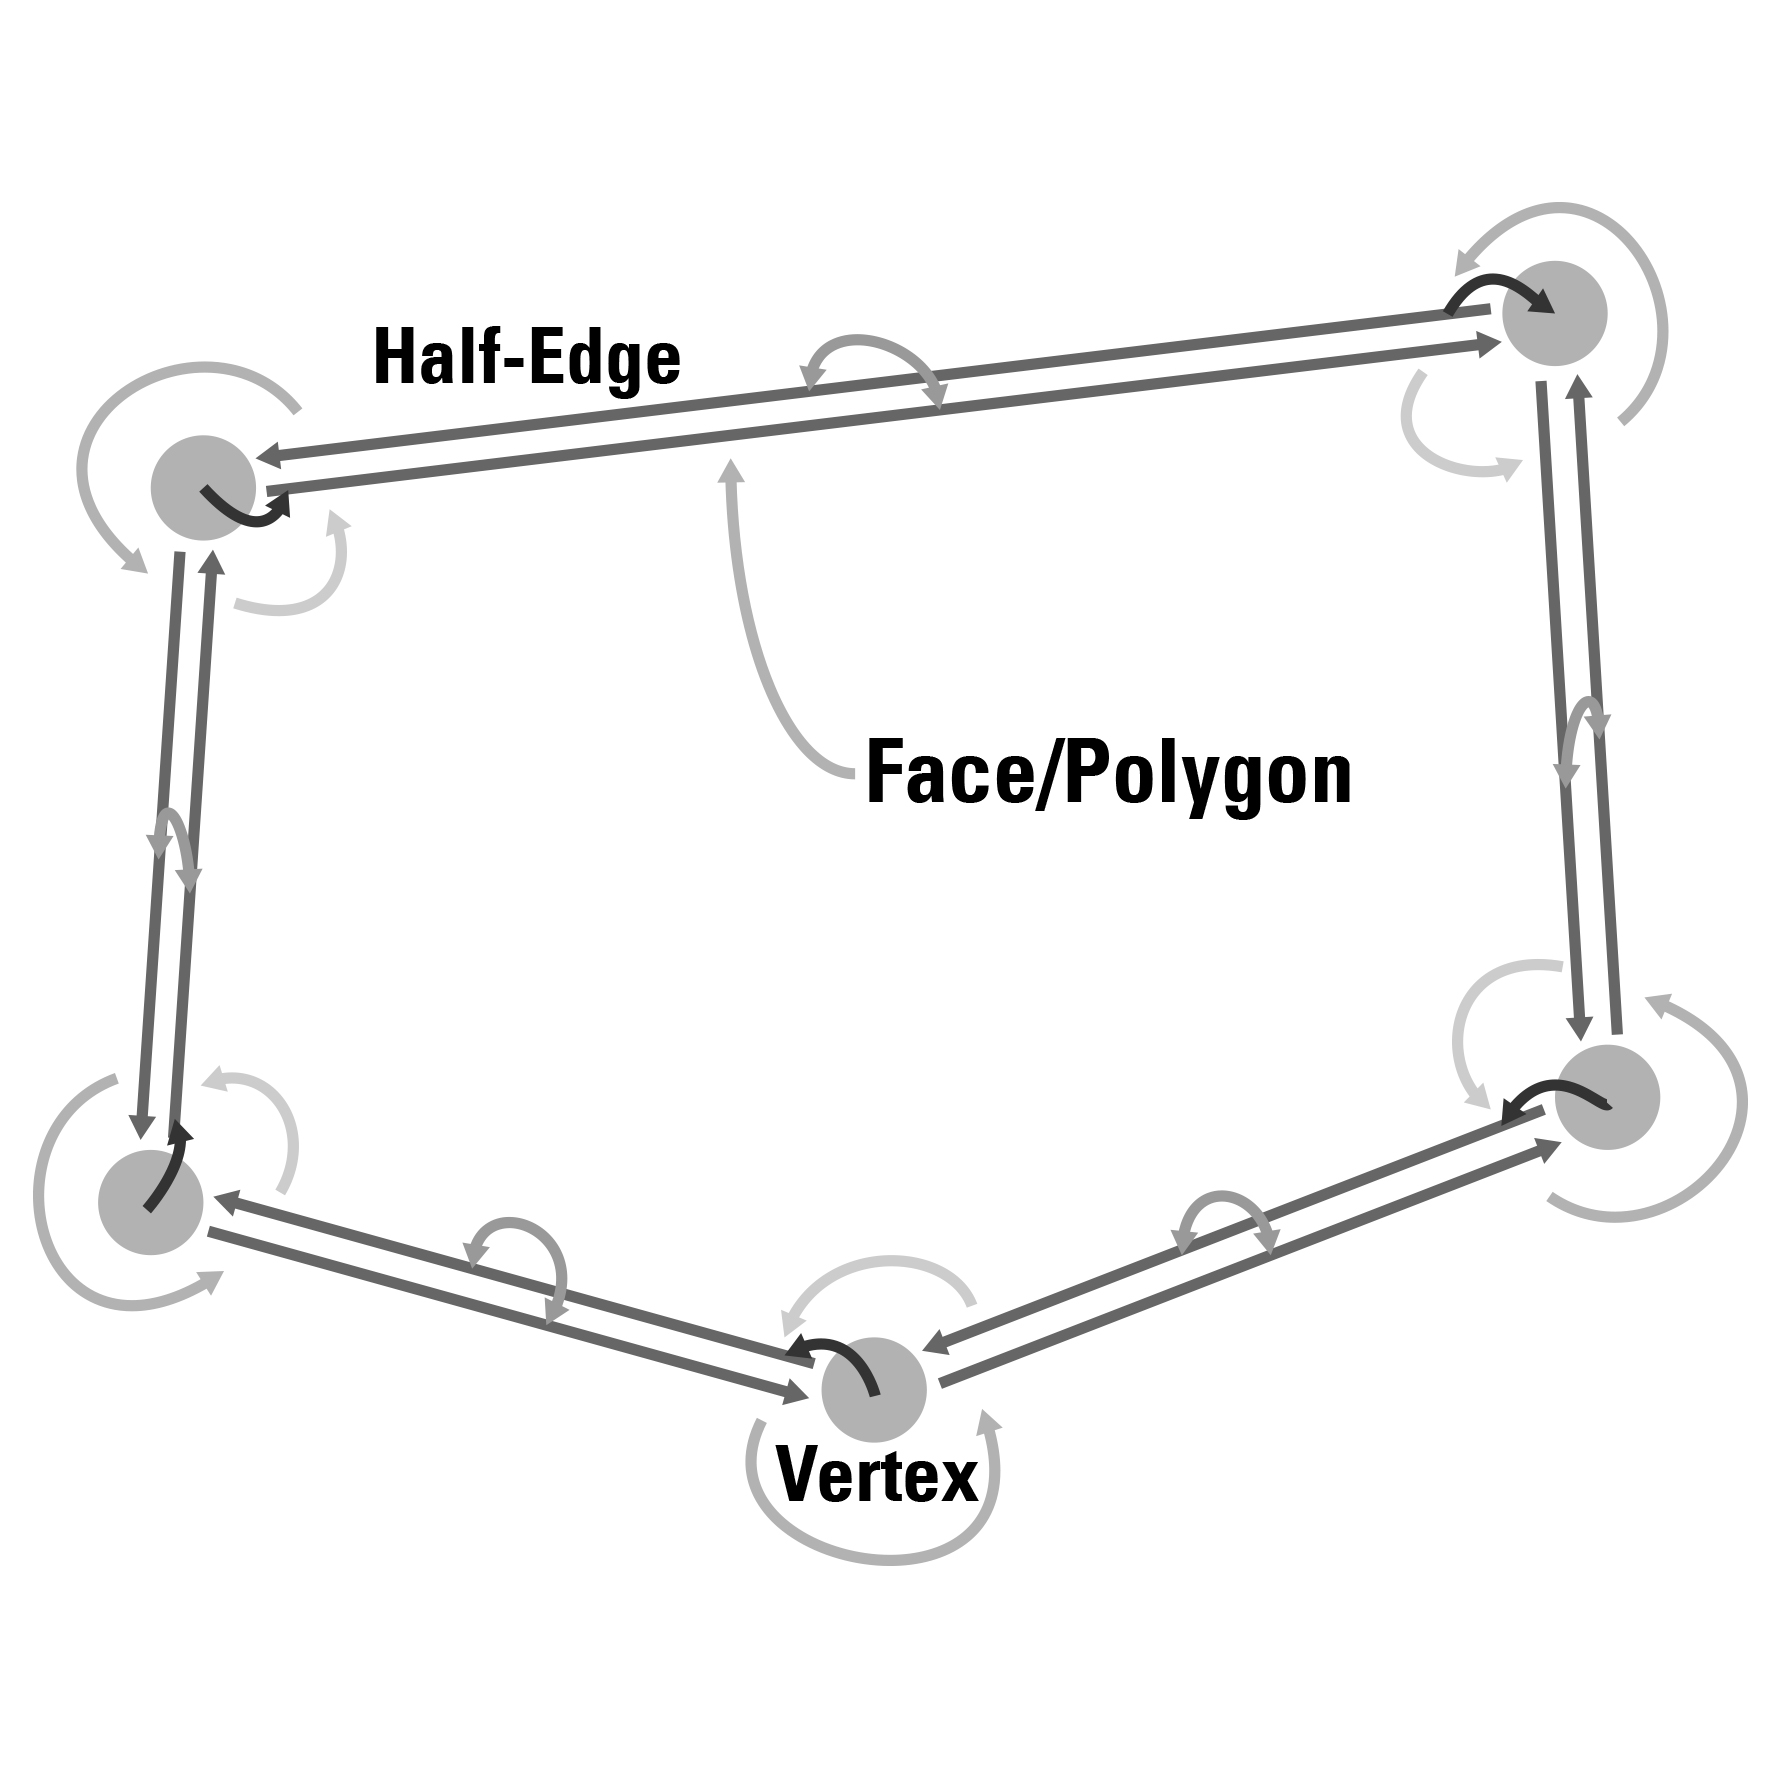
\includegraphics[width=\linewidth]{../Bilder/hesBeziehungen}
\captionof{figure}{Diese Illustration zeigt die Verbindung der data records an einem beliebigen Polygon durch Pfeilverbindungen.}\label{pic:polyConnections} 

An dieser Stelle sei bereits vorweg genommen, dass \LFGS in seiner Implementierung diese data records um ein paar Beziehungen, welche durch die Verbindung zur Echtzeit 3D Engine FUSEE n"otig werden, erweitert.

%Content
		\subsection {Vorteile der \HES}
			%Content
			%TODO rasche geschwindigkeit in iterationen. Beispiel für einen Algorithmus anführen der Kanten eines Polygons sucht oder sonstwie über ein Polygon iteriert.
			% Exemplarisch herausfinden wie das Polygon neben einem Würfel heisst das zwischen zwei vertices liegt.
			Die vielen Verbindungen unter der einzelnen Komponenten in der \HES machen es m"oglich sehr schnelle Iterations Algorithmen zu implementieren. Die Normale eines Faces kann sehr effizient berechnet werden. Es k"onnen auch die Normalen f"ur beliebige Faces unabh"angig vom Rest des Meshes berechnet werden. Dazu ben"otigt man f"ur den Algorithmus nur ein Face als Start Punkt. Der Algorithmus selbst kann f"ur jedes Face der gleiche bleiben.

Subdivision Surface Algorithmen wie Catmull-Clark oder Loop k"onnen mit der Datenstruktur besonders gut realisiert werden. Catmull-Clar ben"otigt dazu ein Mesh aus Quads w"ahrend man mit Loop ein Mesh aus Triangles verarbeiten k"onnte. Beide Mesh Typen, Quads und Triangles, werden vom \LFGS Projekt unterst"utzt. Die FUSEE Engine, in welche das \LFGS Projekt integriert ist, kann im Moment allerdings nur mit Meshes bestehend aus Triangles arbeiten. Aber auch das ist durch die M"oglichkeit der schnellen Iterationen auf der \HES kein Problem.

Die \HES ist also grunds"atzlich sehr flexibel. Es bedingt praktisch nicht, dass jedes Face eines Meshes gleich gro"s ist. \LFG allerdings, in seiner jetzigen Form, erwartet entweder Triangulated Meshes oder Meshes aus Quadlaterals (Quads). Dies ist dem Umstand geschuldet, dass ein Mesh zur weiteren Verwendung in FUSEE konvertiert und verarbeitet werden muss.
		\subsection {Nachteile der \HES}
			%Content
Es gibt selbst in einer so flexiblen Datenstruktur wie der \HES Nachteile die w"ahrend der Planungsphase oder Implementierung auftreten k"onnen.
			Durch ihren Aufbau und die verschiedenen Verbindung welche w"ahrend einer Initialisierung aufgebaut werden m"ussen ist die Datenstruktur sehr komplex. Es erfordert einiges an Zeit und "Uberlegungen das System f"ur eine Implementierung so zu konstrurieren dass es alle Anforderungen an eine 3D Echtzeitdatenstruktur erf"ullt. Vor einer Implementierung der \HES sollte also gut "uberlegt sein ob sie f"ur das aufkommende Probleme eine vern"unftige L"osung darstellt. In \LFGS ist die Datenstruktur eine sehr elegante L"osung. Sie ist hinreichend flexibel und gerade noch maximal komplex um eine m"ogliche L"osung f"ur die Problemstellung "`(Editierbare) Echtzeit 3D Datenstruktur"' darzustellen. Es sollte also darauf geachtet werden die \HES nicht als Universall"osung zu betrachten. Wenn ich nur einige wenige Algorithmen oder Operationen auf einem Mesh ausf"uhren m"ochte, so gibt es m"oglicherweise eine effizientere und schnellere Datenstruktur um dies zu bewerkstelligen.

Ein auff"alliger Unterschied zu einfacheren Face basierten Datenstrukturen ist der massiv erh"ohte Overhead der bei der Erstellung der Datenstruktur entsteht. Im n"achsten Abschnitt m"ochte diese Arbeit ein kleines Beispiel vorweisen und exemplarisch den Speicherverbrauch der \HES bestimmen.

\subsubsection {Speicherverbrauch im Gegensatz zu Face basierten Datenstrukturen}
			%Content
			Der Overhead der bei der Repr"asentation eines Meshes f"ur eine \HES entsteht ist um einiges h"oher als der Overhead einer Face basierten L"osung. Sollte man also nur einfache Aufgaben auf einem Mesh erledigen wollen oder einige wenige Operationen nur einmal ausf"uhren wollen so w"are es wohl ratsam eine andere Datenstruktur daf"ur zu suchen. Allerdings ist es heute in der Computergrafik meistens so, dass wir gen"ugend Speicherplatz im Prim"arspeicher unserer Rechner und Grafikkarten zur verf"ugung haben um diesen Umstanz zu verschmerzen.
Hier eine Beispielhafte Berechung des Datenverbrauchs.

Man gehe davon aus jedes gespeicherte Element (Daten in Form von Vertices, Faces, Edges, Half-Edges) wird mit 32bit repr"asentiert und jeder Zeiger (Pointer) wird mit 8bit repr"asentiert dann k"onnte man den Speicherverbrauch eines einfachen sechs Seitigen W"urfels wie folgt beschreiben.

So stellt die\HES einen W"urfel dar:
\begin{itemize}
\item 24 Half-Edges jede beansprucht 32 bit
	\begin{enumerate}
    	\item Ein Vertex Pointer mit 8bit
    	\item Ein Twin Pointer mit 8bit
    	\item Ein Next Pointer mit 8bit
    	\item Ein Face Pointer mit 8bit
	\end{enumerate}
\item 12 Edges jede beansprucht 32 bit
	\begin{enumerate}
    	\item Zwei Half-Edge Pointer mit je 8bit
	\end{enumerate}
\item 6 Faces jedes beansprucht 32 bit
	\begin{enumerate}
    	\item Half-Edge Pointer eins mit 8bit
	\end{enumerate}
\item 8 Vertices jeder beansprucht 32 bit
	\begin{enumerate}
    	\item Half-Edge Pointer eins mit 8bit
	\end{enumerate}
\end{itemize}

Daraus w"urden sich nun folgende Berechnungen ergeben:

	Half-Edge Datenmenge: \begin{math}24 * (32bit+ 8bit + 8bit + 8bit + 8bit) = 1536bit\end{math}
	\\
	Edge Datenmenge: \begin{math}12 * (32bit + 8bit + 8bit) = 576bit\end{math}
	\\
	Face Datenmenge: \begin{math}6 * (32bit + 8bit) = 240bit\end{math}
	\\
	Vertex Datenmenge: \begin{math}8 * (32bit + 8bit) = 320bit\end{math}

	In Summe sind das 2672bit = 334 Byte.
\newline

Eine Face basierte L"osung w"urde den W"urfel so darstellen:
\begin{itemize}
\item 6 Faces jedes beansprucht 32 bit
	\begin{enumerate}
    	\item Vier Vertex Pointer mit 8bit pro Face
	\end{enumerate}
\item 8 Vertices jeder beansprucht 32 bit
\end{itemize}

Der Datenverbrauch w"urde wie folgt berechnet:

	Face Datenmenge: \begin{math}6 * (32bit + 8bit + 8bit + 8bit + 8bit) = 384bit\end{math}
	\\
	Vertex Datenmenge: \begin{math}8 * 32bit = 256bit\end{math}

	In Summe sind das 640bit = 80Byte.
\newline

Das Beispiel zeigt also, dass bei einem einfachen Mesh der Speicherverbrauch der \HES um das ca. 4 fache h"oher liegt als der Verbrauch einer Face basierten L"osung. Wie die \HES das aber wieder ausgleicht ist dem Abschnitt "`Vorteile der HES"' zu entnehmen.
	\section {Aktueller Forschungsstatus}
		%Content
		% TODO
		% Erwähnen und einordnen von OpenMesh, zusätzlich noch mal eben recherchieren ob es neue implementierungen der dcel oder der hes gibt welche sich in einer 3d engine oder dergleichen bewegen.
		\subsection {Probleme der aktuellen Forschung}
			%Content
			% TODO
			% Hängt stark vom oberen Abschnitt ab.
	\section {Einführung zu LINQ in \CS}
		%Content
		Language Integrated Query, kurz LINQ und zu deutsch Sprachintegrierte Abfrage, funktioniert ab \CSS 3.0 und ist ein Feature von Microsofts .NET Paket. LINQ ist also ein Produkt von Microsoft und erinnert auf den ersten Blick in seinem syntaktischen und semantischem Aufbau stark an das Open Source Projekt MySQL welches aktuell (Stand Juli 2013) von der Oracle Corporation betreut wird. Beide Projekte unterscheiden sich jedoch wesentlich. LINQ ist in erster Linie ein Feature, dass direkt auf Objekten arbeitet wohingegen MySQL auf relationale Daten angewendet wird. Allerdings kann LINQ viel mehr als das.

LINQ kann als Layer und Bindeglied zwischen Collections aus Daten und den Programmiersprachen des .NET Frameworks betrachtet werden. Es ist hierbei m"oglich LINQ in verschiedenen Bereichen zu nutzen. Es arbeitet sowohl wie bereits erw"ahnt auf Collections aus Daten wie z.B. Listen aus Objekten die sich bereits im Hauptspeicher befinden oder fungiert als Bindeglied zu SQL um Daten aus einem Persistenten Medium auszulesen. Es kann aber auch dazu verwendet werden mit XML Datens"atzen bzw. Dokumenten zu arbeiten ist aber auch in der Lage mit Filesystemen und anderen Datenquellen zu interagieren. Das bedeutet dass LINQ sich nicht grunds"atzlich auf die vorher genannten M"oglichkeiten beschr"ankt sondern offen ist f"ur viele Arten von Daten. Weitere sind LINQ to DataSet und LINQ to SharePoint auf die hier mangels Relevanz zum Projekt nicht weiter eingegangen wird.

Diese Arbeit besch"aftigt sich also haupts"achlich mit dem LINQ Provider (LINQ Anbieter) LINQ to Objects da sich die zu verarbeitenden Daten w"ahrend der Bearbeitungszeit mit LINQ bereits im Speicher des Rechners befinden. Wie erw"ahnt, ist LINQ ein Layer f"ur die Programmiersprachen von .NET und kann deswegen nicht nur in \CSS verwendet werden wie hier, sondern auch in Microsofts VB.NET. Dieses Projekt beschr"ankt sich auf \CSS als Programmiersprache, weswegen auch alle folgenden Codebeispiele in \CSS geschrieben sind. Ein weiterer nicht zu verachtender Vorteil von LINQ im Gegensatz zu den meisten Implementationen von SQL Statements ist, dass die Statemtents vom \CSS compiler zum Zeitpunkt der Kompilierung auf syntaktische Korrektheit gepr"uft werden und der Benutzer vom IntelliSense System von Visual Studio wertvolle Hinweise w"ahrend der Generierung von LINQ Statements erh"alt.
		%Content
		\subsection {Was ist LINQ to Objects genau? }
		%Content
		LINQ to Objects wie in diesem Projekt verwendet, erfordert zur Benutzung erst einmal die grunds"atzliche Eigenschaft des Datensatzes eine Collection zu sein. Jede Collection aus Objekten auf die LINQ to objects angewendet wird muss also die Schnittstelle IEnumerable\GTS implementieren. Diese Objekte werden im LINQ Vokabular dann als Sequences bezeichnet. In dieser Arbeit werden fast aussschliesslich die generischen Collections von \CSS verwendet welche grunds"atzlich auch alle das generische IEnumerable\GTS Interface implementieren. Der am meisten verwendete Datentyp in dieser Arbeit ist die generischen Implementierung von List\GT.

Eine LINQ to object Abfrage besteht immer aus drei Abfrageoperationen
\begin{itemize}
\item Bereitstellen einer Datenquelle
\item Erstellen einer LINQ Abfrage
\item Ausführen der LINQ Abfrage auf der Datenquelle mithilfe einer foreach() Anweisung
\end{itemize}
Das besondere an der Formulierung von LINQ Statements ist, dass sie zum Zeitpunkt ihrer Erstellung noch keine Daten der Datenquelle abfragen sondern erst zum Ausf"uhrungszeitpunkt des Statements damit beginnen. Das ist sehr praktisch, denn dadurch k"onnen einmal in einer Abfrage erstellte Statements wiederverwertet werden. Eine LINQ Abfrage Variable speichert nie das Ergebnis einer Abfrage. Durch diesen Umstand ist es möglich, einen Datensatz zu unterschiedlichen Zeitpunkten abzufragen. Eventuell "andert sich auch das Ergebnis der Abfrage wenn man davon ausgeht dass sich die Collection der Daten "uber die Zeit ver"andert. Trotzdem wird immer nch die semantisch gleiche Abfrage verwendet. LINQ Abfragen werden also mit einer Verz"ogerung schlussendlich in einer foreach() Anweisung ausgef"uhrt. Dabei durchl"auft die foreach() Anweisung Syntaktisch die Query oder Statement variable und nicht die Collection der Daten.
\\
Hier folgt ein Beispiel welches eine einfache LINQ Abfrage auf einen einfachen Array Datensatz der IEnumerable\GTS implementiert darstellt.
\lstinputlisting
			[caption={LINQeasyQuery.cs - Einfaches LINQ Abfrage Beispiel}, label=code:linqeasyquery]
			{../Codebeispiele/LINQeasyQuery.cs}

Ein Statement kann jedoch auch erzwungen direkt ausgef"uhrt werden. Durch einen direkten Aufruf der Methoden toList\GTS oder toArray\GTS auf dem Statement.
%\caption[Foo Bar.]{Foo Bar. Redrawn from \protect\cite{Baz}.}
\lstinputlisting
			[caption={LINQdirectQueryList.cs - Einfaches direktes LINQ Abfrage Beispiel} \protect\cite{MicrosoftCReferenz.2013}, label=code:linqdirectquery]
			{../Codebeispiele/LINQdirectQueryList.cs}
		%Content
		\subsection {Abfragesyntax in LINQ}
		Was im vorigen Absatz als LINQ Statement bezeichnet wurde ist ein LINQ Statement geschrieben in der Abfragesyntax. Diese Syntax zeichnet sich durch einfache Lesbarkeit und einfache Zug"anglichkeit aus. Zur Kompilierzeit wird diese Syntax vom Compiler in die so genannte Methodensyntax "ubersetzt. Die beiden syntaktischen Varianten sind Semantisch identisch auch wenn sie sich auf den ersten Blick sehr unterscheiden.
		%Content
		\subsection {Methodensyntax in LINQ}
		Die Methodensyntax in LINQ unterscheidet sich von der Abfragesyntax dadurch, dass anstatt fester keywords wie where, from und select um eine Abfrage zu formen Lambda Ausdr"ucke verwendet werden (Lambda Ausdr"ucke werden im n"achsten Abschnitt n"aher erleutert). In der Referenzdokumentation zu LINQ (Stand Juli 2013) \cite{MicrosoftCReferenz.2013} wird haupts"achlich diese Art der Syntax verwendet. Aus den dort aufgef"uhrten Typen wird in dieser Arbeit sehr h"aufig der Enumerable Typ verwendet.
\\
Hier ein Vergleich der beiden Syntaktischen M"oglichkeiten zum erstellen von LINQ Statements.
\lstinputlisting
			[caption={LINQzweiSynt.cs - Zwei syntaktische M"oglichkeiten} \protect\cite{MicrosoftCReferenz.2013}, label=code:linqzweisynt]
			{../Codebeispiele/LINQzweiSynt.cs}
		%Content
	\section {Einführung zu Lambda in \CS}
		%Content
		Lambda Ausdr"ucke in \CSS sind Anonymen Funktionen sehr "ahnlich. In dieser Arbeit wurden Lambda Ausdr"ucke haupts"achlich in LINQ Statemens verwendet. Syntaktisch ist diese Art Funktionen zu schreiben sehr simpel gestrickt. Das Lambda Zeichen in \CSS wird als \LAM dargestellt. Es folgt immer der Parameterliste und sollte nicht mit den Vergleichsoperatoren \textgreater = und \textless = verwechselt werden. Das Lamba Zeichen bedeutet hier soviel wie "`wechselt zu"' oder "`wird zu"' und steht Links des gew"unschten Ausdrucks.
		%Content
		\subsection {Lambda Ausdr"ucke in Verbindung mit LINQ}
Wie bereits beschrieben werden Lambda Ausdr"ucke  in verbindung mit LINQ in der Methodensyntax von LINQ verwendet. Diese Syntax wird meist benutzt um Standardabfrageoperatoren wie Collection.Select(lambda hier) Collection.Where(lambda hier) und Collection.All(lambda hier) zu verwenden. In dieser Arbeit wird der Standardoperator Select() am h"aufigsten verwendet. Select() wenden den angegebenen Lambda Ausdruck auf jedes Element der Collection an auf die der Select operator angewendet wird und gibt falls vorhanden ein Ergebnis zur"uck. Siehe Listing \ref{code:lambdaeasy}
\lstinputlisting
			[caption={LambdaEasy.cs - Einfacher Lambda Ausdruck}, label=code:lambdaeasy]
			{../Codebeispiele/LambdaEasy.cs}
%%%%%%
%	Einführung / Einleitung ENDE
%%%%%%



%%%%%%
%	Hauptteil START
%%%%%%

\chapter {Hauptteil}
	\section {Gegenüberstellung nativer (OpenMesh.org) und gemanagter Implementierungen der Half-Edge Data Structure}
		%Content	
		%Content
	\section {Geschwindigkeitsunterschiede von nativem und \CSS Code}
		%Content
		%Content
	\section {Die Vorteile in der Entwicklung mit managed Programmiersprachen}\label{sec:VorteileManaged}
		%Content
Durch die enge Verkn"upfung von \LFGS mit der FUSEE Engine war es nat"urlich n"otig das Projekt in der gleichen Programmiersprache wie FUSEE zu implementieren um eine Kommunikation der beiden Projekte zu erlauben. Obwohl die .NET basis hier nat"urlich Spielraum f"ur Entscheidungen zugunsten VB.NET gelassen h"atte. Sinnvoll w"are das nat"urlich nicht gewesen. Hier soll jetzt kurz gekl"art werden was "`Managed Code"' genau bietet und warum \LFGS in einer solchen Sprache wie \CSS implementiert wurde. Nat"urlich einmal davon abgesehen, dass \LFGS mithilfe von LINQ implementiert wurde und LINQ eine der S"aulen des Projekts darstellt.

		Managed Code bietet einem Entwickler viele verschiedene Vorteile im Gegensatz zur Entwicklung in einer Nativen Programmiersprache. Im Hinblick auf die \HES sollte besonders das Speichermanagement und die Pointer Verwaltung betrachtet werden. Durch die in \CSS implementierte Garbage Collection ist der Programmierer von der Aufgabe befreit das Speichermanagement selbst zu verwalten. Das bietet einen gro"sen Vorteil in der schnellen Entwicklung von Programmiersprachen. Managed Code ist f"ur viele Entwickler einfacher zu schreiben als native Code in Sprachen wie z.B. C++.

Im Hinblick auf \LFGS f"allt durch die Nutzung von \CSS einiges an Arbeit weg. Nicht mehr gebrauchte tempor"are Listen, von denen es einige im Projekt gibt und Objekte werden automatisch durch die Garbage Collection aufger"aumt und es kommt sehr selten bis kaum zu Memory Leaks durch Programmier- oder Laufzeitfehler. Es ist so wesentlich einfacher externen Nutzern einen Zugang auf den Code des Projekts zu erm"oglichen ohne dass sie Gefahr laufen die Integrit"at der Datenstruktur durch Pointer Manipulationen zu gef"ahrden. \CSS bietet hier also ein gewisses Ma"s an Sicherheit f"ur das System.

Ein weiterer Pluspunkt ist nat"urlich, dass sich bereits viele Entwickler und Studenten der Hochschule Furtwangen die sp"ater m"oglicherweise die FUSEE Engine verwenden m"ochten bereits mit \CSS oder Java, welches \CSS zumindest Syntaktisch sehr "ahnelt, auskennen.
		%Content
\section {Das Software Projekt LINQ For Geometry}
		%Content
Das Softwareprojekt \LFGS (kurz LFG) welches im Rahmen dieser Thesis Arbeit entworfen und implementiert wurde, stellt eine Umsetzung der \HES zum Handling dreidimensionaler Meshes dar. \LFGS hat darüber hinaus den Anspruch die Datenstruktur durch eine anprogrammierung mit LINQ Ausdr"ucken bearbeitbar zu machen. Es bietet einen Converter in das von der FUSEE Engine benutze Mesh Format und kann in Echtzeit Geometrische Operationen auf einem in der Datenstruktur gespeichertem Mesh ausf"uhren. \LFG wurde Anfangs als eigenst"andiges Projekt begonnen. Im sp"ateren Verlauf wurde es in die FUSEE Engine integriert um dort wahlweise Meshes in der \HES im Speicher bereit zu halten. Das \LFGS Projekt ist von FUSEE nicht abh"angig. Es benutzt ledigleich ein Paar der Datentypen aus der Mathematik Bibliothek von FUSEE und den Mesh Datentypen welchen \LFGS aufgrund der converter Funktion nach FUSEE Mesh kennen muss. \LFGS w"are also nach Wunsch auf andere Engines oder Programme mit wenigen Anpassungen portabel.

\LFGS erweitert die \HES um ein paar Funktionen um die korrekte Darstellung von Meshes in FUSEE zu gew"ahrleisten. Dazu z"ahlen Erweiterungen der an den Kanten und Faces gespeicherten Informationen um UV Textur Koordinaten und Face- und Vertex Normalen im Mesh zu speichern.
Zus"atzlich ist es in der Lage Kanten zu verarbeiten die an mehr als 2 Polygone grenzen. Diese L"osing ist allerdings zum Zeitpunkt Juni 2013 nur als Notl"osung zu betrachten und das massive Edge Sharing (Teilen von Kanten mit vielen Faces) sollte wenn m"oglich bereits beim modellieren eines Meshes vermieden werden.
\newline

In den n"achsten Abschnitten steht die Implementierung von \LFG im Vordergrund und versucht ein Umfassendes Bild zu vermitteln wie genau die \HES mit Hilfe von LINQ und Lambda Support in \CSS aufgebaut werden kann.
\newline
		%Content
		\subsection {Konzept zu \LFG}
			%Content
			%Content
			\subsubsection {Der Link von LINQ zur \HES}
				%Content
				%Content
		\subsection {Warum die Programmiersprache \CSS f"ur \LFG?}
			%Content
			Wie bereits  im oberen Abschnitt \ref{sec:VorteileManaged} angeschnitten, wurde \LFGS daf"ur konzipiert mit der FUSEE Engine zusammen zu arbeiten. \LFGS bietet hierbei eine neue Geometry Objekt Klasse f"ur die FUSEE Engine an, ohne die tats"achliche zu "uberschreiben. Laut aktuellem Stand kann der Benutzer beider Projekte sich also entscheiden welche Meshes er gerne in der \HES laden m"ochte und f"ur welche es gen"ugt sie als Face basiertes Mesh im Speicher zu halten.

Damit \LFGS auf diese Art mit der FUSEE Engine kommunizieren kann musste eine gemeinsame Schnittstelle evaluiert werden. Weil beide Projekte die .NET Plattform benutzen und FUSEE in \CSS geschrieben wurde war es naheliegend f"ur \LFGS auch \CSS zu benutzen und da der LINQ Layer ein Produkt von .NET ist, war \CSS die wohl beste Wahl um beide Projekte zusammen zu bringen.
			%Content
		\subsection {Furtwangen University Simulation and Entertainment Engine (FUSEE)}
			%Content
			Die Furtwangen University Simulation and Entertainment Engine (kurz FUSEE) ist eine Open Source 3D Echtzeit Engine mit einem Schwerpunkt auf Multiplattform Unterstützung. Entwickelt wurde sie von einer Projektgruppe an der Hochschule Furtwangen unter der Leitung von Herrn Prof. M"uller an der Fakult"at Digitale Medien.Von der aktuellen Version 0.5 werden folgende Plattformen unterst"utzt.
\begin{itemize}
\item Windows OS
\item Linux OS
\item Android OS
\item Die Android Konsole OUYA
\item Der Chrome Browser
\item Der Firefox Browser
\end{itemize}

Um eine Linux und Android Unterst"utzung zu erreichen ist das Projekt mit Mono, einer .NET Open Source Implementierung, kompatibel. Sogar einen export nach JavaScript durch den JSIL Compiler von Kevin Gadd ist m"oglich. Somit ist FUSEE ohne weitere Plugins im Browser lauff"ahig.

Hier eine Liste der bereits umgesetzten Features in der Version 0.5:
\begin{itemize}
\item Multitexturing
\item Ein standard Set an Shadern ist verf"ugbar
\item Benutzerdefinierte Shader sind m"oglich
\item Ein Scene Management wird unterst"utzt
\item Sound in Browsern und Betriebssystemen vorhanden
\end{itemize}

\LFGS ist als Sideproject in einen FUSEE Branch integiert. Nach aktuellem Stand (Juli 2013) kann man sich als Benutzer entscheiden ob man dann ein Modell mit dem in FUSEE integrierten Mesh System oder mit dem \HES Geometry System von \LFGS laden m"ochte.

Weitere Informationen "uber die FUSEE Engine sind auf der offiziellen Homepage (http://fusee3d.org/) oder "uber GitHub (https://github.com/FUSEEProjectTeam/Fusee) erh"ltlich.
Quelle http://fusee3d.org/about/) (Stand 19.07.2013)

			%Content
	\section {Der Import von Geometriedaten im „Wavefront Object“ Format}
		%Content
		%Content
		\subsection {Warum das Wavefront Object Format}
			%Content
			%Content
		\subsection {Face basierter Import - Edge basiertes Handling}
			%Content
			%Content
		\subsection {Importer für das Wavefront Format}
			%Content
			%Content
	\section {Initialisierungsablauf}
			%Content
			%Content
		\subsection {UML Diagramme zum Initialisierungslauf}
				%Content
				%Content
	\section {Implementierung und Funktion der Handler für die einzelnen Komponenten der HES}
		\subsection {Beispiel eines Handler Konstruktes und seiner Implementierung}
		%Content
Die Handler Konstrukte "`Structs"' in dieser Arbeit, welcher Art auch immer, können vereinfacht gesagt als Zeiger auf Datens"atze von realen Daten betrachtet werden.
\lstinputlisting
			[caption={HandleHalf-Edge.cs - Variablen Deklaration des "`Zeigers"'}, label=code:hhezeiger, firstline=21, lastline=21]
			{../../HFU_FUSEE/Fusee/src/Engine/LinqForGeometry/LinqForGeometry.Core/src/Handles/HandleHalfEdge.cs}
Sie enthalten nur einen Index als Zeiger und sehr wenige Funktionen. Ein Handler speichert zur Laufzeit pro Instanz einen Index auf den realen Datensatz f"ur den er einen Handle darstellt. Handler Structs gibt es f"ur Edges, Half-Edges, Faces, FaceNormals, Vertices, VertexNormals und VertexUVs. Sie unterscheiden sich hierbei nur durch die Namensgebung der Structs und der Konstrukturen.
Ein Handler Struct stellt eine implizite Konvertierung des Handlers, siehe Listing \ref{code:hhecast}, in den Datentypen Integer (int) zur Verfügung.
\lstinputlisting
			[caption={HandleHalf-Edge.cs - Impliziter cast nach Integer}, label=code:hhecast, firstline=37, lastline=40]
			{../../HFU_FUSEE/Fusee/src/Engine/LinqForGeometry/LinqForGeometry.Core/src/Handles/HandleHalfEdge.cs}

Zus"atzlich kann der Entwickler jederzeit abfragen ob der aktuell verwendete Handler schon als valide betrachtet werden kann. Hierzu Listing \ref{code:isvalid} betrachten. Ein Handler ist dann valide, wenn sein Index nicht kleiner als 0 ist. In dieser Arbeit werden einstweilen Handler initialisiert f"ur die zum Zeitpunkt der Initialisierung noch kein Index zur Speicherung bereit steht. Diese vorerst nicht validen Handler werden dann mit dem Wert -1 initialisiert und sind somit zu diesem Zeitpunkt als nicht valide also nicht verwendbar zu betrachten. Um diese sp"ater im Programm zu benutzen, muss also noch der korrekte Index, meistens der Wert einer Count Funktion auf einer Liste eingef"ugt werden.
\lstinputlisting
			[caption={HandleHalf-Edge.cs - Is Valid?}, label=code:isvalid, firstline=45, lastline=48]
			{../../HFU_FUSEE/Fusee/src/Engine/LinqForGeometry/LinqForGeometry.Core/src/Handles/HandleHalfEdge.cs}

Eine Besonderheit der Handler ist die mit "`internal"' gekennzeichnete Deklaration der Indizes. Siehe hierzu Listing \ref{code:hheinternal}. Durch das "`internal"' \CSS Schl"usselwort k"onnen die Handler nur aus der jeweiligen gleichen Assembly angesprochen und ver"andert werden. Dies verhindert einen unbefugten oder unabsichtlichen Fremdzugriff von Au"sen. W"ahrend der Laufzeit wird also die Konsistenz der Datenstruktur in sich gesch"utzt um so das Programm vor Abst"urzen durch Zeiger Fehler zu sch"utzen.
\lstinputlisting
			[caption={HandleHalf-Edge.cs - Deklarationen als internal}, label=code:hheinternal, firstline=21, lastline=21]
			{../../HFU_FUSEE/Fusee/src/Engine/LinqForGeometry/LinqForGeometry.Core/src/Handles/HandleHalfEdge.cs}

\begin{quote}{\dq}Der interne Zugriff wird h{\"a}ufig in komponentenbasierter Entwicklung verwendet, da er einer Gruppe von Komponenten erm{\"o}glicht, in einer nicht {\"o}ffentlichen Weise zusammenzuwirken, ohne dem Rest des Anwendungscodes zug{\"a}nglich zu sein.{\dq} \cite{MicrosoftCReferenz.2013}\end{quote}


Die vollst"andige Implementierung dieses Structs und aller sieben weiteren kann im Visual Studio 2010 Projekt auf dem diese Arbeit aufbaut unter folgender Verzeichnisstruktur betrachtet werden. "`LinqForGeometry/LinqForGeometry.Core/src/Handles"'
		%Content

\section {Pointer Container und ihre Aufgabe in \LFG}
		%Content
		Pointer Container in \LFGS sind \CSS Structures und existieren f"ur jeden in der Datenstruktur essentiellen Datentypen und geh"oren zum Kern Projekt (LinqForGeometry.Core) des \LFGS Projekts. Zu den Containern z"ahlen Half-Edges Container, Edge container, Face Container und Vertex Container. Ein Pointer Container wird f"ur jeden Datensatz der in die Datenstruktur eingef"ugt wird initialisiert und in einer Liste gespeichert. Jeder Container enth"alt, den Spezifikationen der \HES folgend Handles auf andere eingepflegte oder in kurzer Zeit einzupflegende Datens"atze z.B. durch eine mathematische Operation (welche den voraussichtlichen Index eines einzuf"ugenden Datensatzes berechnet). Pointer Container sind sozusagen die Gebilde welche die Half-Edge Datenstruktur aufspannen und ihre Eigenschaften im Speicher vorhalten. M"ochte man ein gespeichertes Mesh transformieren so sind alle Operationen die vorgenommen werden "Anderungen an den Pointer Containern bzw. den in ihnen enthaltenen Daten. Pointer Container sind also die Basis des ganzen Programms. Durch die Gegebenheiten der Implementierung von List<T> (Generic Lists) in \CSS ist es leider nicht m"oglich die Container bei "Anderungen direkt in einer Liste zu manipulieren. Jeder Container muss erst aus der Liste kopiert werden um ihn dann zu "andern und anschliessen an der gleichen Stelle wieder einzuf"ugen. N"otig hierzu ist, dass der Index des Containers in der jeweiligen Liste bekannt ist. Hierzu ein kleines Beispiel welches die Erkl"arung etwas erl"autern soll.
\lstinputlisting
			[caption={PtrContExample1.cs - Manipulation eines Pointer Containers}, label=code:ptrcontmanip]
			{../Codebeispiele/PtrContExample1.cs}
		%Content
\subsection {Half-Edges Pointer-Container}
%Content
			Der Half-Edge Pointer Container, in \LFGS class HEdgePtrCont, speichert alle Informationen die laut \HES an einer Half-Edge anliegen m"ussen. Die zugeh"orige Datei im \LFGS Projekt ist "`HEdgePtrCont.cs"'.
\begin{itemize}
\item Ein HandleHalfEdge \_he; (auf die Twin Half-Edge)
\item Ein HandleHalfEdge \_nhe; (auf die n"achste Half-Edge im Uhrzeigersinn)
\item Ein HandleVertex \_v; (auf den Vertex auf den die Half-Edge zeigt)
\item Ein HandleFace \_f; (auf das zugeh"orige Face)
\end{itemize}

In der Implementierung von \LFGS werden an einer Half-Edge noch zus"atzliche Handler Informationen f"ur die Verwendung und Konvertierung des Meshes in und nach FUSEE gespeichert.

\begin{itemize}
\item HandleVertexNormal \_vn; (auf die Vertex Normale eines Vertex)
\item HandleVertexUV \_vuv; (auf die UV Texture Koordinaten eines Vertex)
\end{itemize}

Da jede Half-Edge auch eine Verbindung zum Vertex hat auf den sie zeigt ist es sehr praktisch an ihr auch die zus"atzlichen Informationen zu speichern die der Vertex in FUSEE ben"otigt. Es wird also ein Index auf die Vertex Normale im Speicher zum angesprochenen Vertex gespeichert. Zus"atzlich noch ein Index auf die UV Texture Koordinaten die f"ur den Vertex gelten. So kann die Iteration bei einer sp"ateren Konvertierung der Datenstruktur in ein f"ur FUSEE verst"andliches Mesh Objekt "uberhaupt erst m"oglich gemacht werden. Es w"are mit erheblichem Mehraufwand und wachsendem Speicherverbrauch auch m"oglich gewesen die Informationen an den einzelnen Vertices durch Verkn"upfungen mit Listen welche jeweils die die Daten f"ur einen Vertex speichernzu realisieren, allerdings h"atte das eine regelrechte Aufweichung der Idee der Datenstruktur bedeutet (alle wichtigen Informationen werden an den Half-Edges gespeichert). Zus"atzlich w"are es so wesentlich aufwendiger geworden eine korrekte Kanten und Winkel basierte Vertex Normalen Berechnung pro Vertex pro Face f"ur die in FUSEE vorhandene Beleuchtungsshader zu implementieren wie sie durch diese kleine erweiterung der \HES jetzt bereits in \LFGS vorhanden ist.
		\subsection {Edges Pointer-Container}
			%Content
			Ein Edge Pointer Container, in \LFG zu finden im Struct "`EdgePtrcont.cs"', ist ein Repr"asentation von Kanten in der \HES. Jeder Edge Pointer Container beinhaltet zwei Handles auf Half-Edges.
\begin{itemize}
\item HandleHalfEdge \_he1; (Handle auf die Erste Half-Edge eines Half-Edge Paares)
\item HandleHalfEdge \_he2; (Handle auf die Erste Half-Edge eines Half-Edge Paares)
\end{itemize}
Diese beiden Handles sind ein jeweils zusammengeh"origes Half-Edge Paar. Durch die bereitstellung dieser Edge Pointer Container ist zum Beispiel eine Selektierung von echten Kanten in einem 3D Editor denkbar. Sie dienen ebenfalls als Einstiegspunkt um manipulations Algorithmen auf das gespeicherte Mesh anzuwenden.
			%Content	
		\subsection {Vertices Pointer-Container}
			%Content
			Dadurch, dass in der Half-Edge Datenstruktur alle wichtigen Informationen bereits an jeder Half-Edge gespeichert werden, speichern Vertex Pointer Container lediglich einen Handle auf eine von ihm ausgehende Half-Edge. Da ein Vertex aber meistens mehrere ausgehende Half-Edges besitzt wird der Platz nach dem "first come first serve" Prinzip verteilt. Das bedeutet, dass nur die erste Half-Edge die w"ahrend des Initialisierungslauf an den Vertex angelegt wird an dieser Stelle auch referenziert wird. Durch diesen Handle k"onnen Iteratoren sehr einfach realisiert werden die in anderen Datenstrukturen wie der Face basierten Datenstruktur einiges an Mehraufwand bedeuten w"urden. Als Beispiel soll hier der Sternumlauf Iterator genannt werden. Dieser kann alle eingehenden oder ausgehenden Half-Edges zu einem gegebenen Vertex bestimmen. Hier dargestellt kurz der Ablauf des Iterators f"ur eingehende Half-Edges:
\begin{enumerate}
\item Es wird ein Vertex als Startpunkt erwartet
\item Es wird die ausgehende Half-Edge des Vertex angesprochen (und den Index merkt sich der Algorithmus als Determinante)
\item Es wird die Twin Half-Edge der eben geholten Half-Edge angesprochen
\item Die Twin Half-Edge wird als erste eingehende Half-Edge im Ergebnis Set zwischengespeichert
\item Zu dieser Half-Edge wird jetzt die "`Next"' Half-Edge angesprochen.
\item Ihre Twin Half-Edge ist nun wieder eine eingehende Half-Edge.
\item Ab jetzt wird der Algorithmus ab Schritt 3 wiederholt bis man als Index einer n"achsten Half-Edge die zuvor gespeicherte Determinante erreicht.
\end{enumerate}

So ist es mit ein paar Pointer Spr"ungen m"oglich diesen Algorithmus schnell und effizient durchzuf"uhren. In einer Face basierten Datenstruktur w"are eine solche Operation wegen der fehlenden Beziehungen und Vernetzungen ohne massive "Anderungen der Strukur kaum m"oglich.
			%Content
		\subsection {Faces Pointer-Container}
			%Content
			Laut Definition der \HES speichert ein Face jeweils einen Zeiger auf eine ihm angeh"orige Half-Edge. In \LFG wurde genau das in der Implementierung umgesetzt. Das erleichtert den Einstieg in manipulations Algorithmen wenn der Startpunkt f"ur diese als Face gegeben ist. So ist es einfach die Grenzen (Boundaries) eines Faces und z.B. die das Face umspannenenden Half-Edges, Edges, Vertices oder sogar die benachbarten Faces herauszufinden. \LFGS stellt in seiner Implementierung all diese Iteratoren zur Verf"ugung um damit weitere Algorithmen zu entwerfen.

\begin{itemize}
\item HandleHalfEdge \_h;
\end{itemize}

Zus"atzlich zu den Standards der \HES bietet \LFGS die M"oglichkeit an jedem Face ein Handle auf eine dem Face zugeh"orige Face Normale zu speichern. Diese Face Normale gibt die Richtung des Faces an sollte die Datenstruktur in eine 3D Engine implementiert werden in welcher Backface Culling unterst"utzt und dabei Normalen als Ausrichtungsmerkmal beachtet werden. In \LFG und seiner Implementierung in der FUSEE Engine wird die Face Normale aktuell nur zur Berechnung der Vertex Normalen herangezogen. FUSEE ben"otigt f"ur das Backface Culling lediglich eine Traversierung der Polygone entgegen des Uhrzeigersinns. Diese Besonderheit tritt in Engines auf welche OpenGL als Grafikschnittstelle verwenden.
\begin{itemize}
\item HandleFaceNormal \_fn;
\end{itemize}
			%Content
	\section {Die Geometrie in \LFG}
		%Content
			Das Geometry Objekt ist der Kern des ganzen \LFGS Projekts. Von der Umwandlung eines mit dem Importer eingelesenen Meshes bis zur Speicherung w"ahrend der Laufzeit managed das Geometry Objekt ein komplettes Mesh. Die gespeicherten Daten im Objekt werden in Collections vorgehalten um einen schnellen Zugriff durch Iteratoren zu gew"ahrleisten. Es werden Listen anstelle von Arrays oder "ahnlichem verwendet um die Handhabung von Zugriffen auf die Daten zu erleichtern.

Eine "Ubersicht "uber die gespeicherten und zur Verf"ugung stehenden Collections inklusiver ihrer Zugriffsmodifizierer und Datentypen.
\begin{itemize}
\item Handles auf Pointer Container
	\begin{itemize}
    \item public List<HandleVertex> \_LverticeHndl;
    \item public List<HandleEdge> \_LedgeHndl;
	\item public List<HandleFace> \_LfaceHndl;
	\end{itemize}
\item Pointer Container
	\begin{itemize}
	\item private List<VertexPtrCont> \_LvertexPtrCont;
	\item private List<HEdgePtrCont> \_LhedgePtrCont;
	\item private List<EdgePtrCont> \_LedgePtrCont;
	\item private List<FacePtrCont> \_LfacePtrCont;
	\end{itemize}
\item Reale Daten
	\begin{itemize}
	\item public List<float3> \_LvertexVal;
	\item public List<float3> \_LfaceNormals;
	\item public List<float3> \_LVertexNormals;
	\item private List<float2> \_LuvCoordinates;
	\item private List<float3> \_LvertexValDefault;
	\end{itemize}
\end{itemize}
Diese Listen enthalten alle wichtigen Informationen "uber das in der \HES vorhandene Mesh. Durch Manipulation der darin gespeicherten Daten kann das Mesh ver"andert werden. Alle von \LFGS implementierten Iteratoren und Geometrie Manipulatoren benutzen diese Listen.

Das Geometrie Objekt kann aus dem \LFG.ExternalModul Projekt heraus angesprochen werden um weitere Manipulationsalgorithmen zu erstellen.
\lstinputlisting
			[caption={ExternalModule.cs - Wie wird ein Geometry Objekt im externen Modul verwendet}, label=code:externalModule]
			{../Codebeispiele/ExternalModule.cs}

Das Geometry Object wird hier durch Call by Reference (dargestellt durch das Keyword "`ref"' in \CS) "ubergeben. Diese Methode spart aufgrund der Gr"o"se eines Geometry Objekts und der vielen darin enthaltenen Daten einiges an Zeit und Speicherplatz im Arbeitsspeicher (RAM).

		%Content
		\subsection {Benchmarks zu Laufzeiten des Programms}
			%Content
			%Content
	\section {Anwendungsszenarien von \LFG}
		%Content
	\LFGS kann mit der \HES als Basis f"ur viele Anwendungesgebiete interessant sein. Aktuell ist das System als Ersatz f"ur das in FUSEE integrierte Mesh Konzept eingebettet. Hier l"adt es Meshes aus Wavefront Object Dateien w"ahrend der Laufzeit eines FUSEE Programms in den Speicher und h"alt die Daten bereit. Das Mesh kann dann w"ahrend der Laufzeit durch verschiedene Methoden manipuliert werden. Allerdings sind weitere Einsatzgebiete denkbar und teilweise sogar angedacht.
Das System k"onnte es zum Beispiel m"oglich machen Meshes zur Laufzeit eines Spiels zu ver"andern. Dabei w"are es denkbar Konstruktion oder Destruktion in einer Echtzeit Spielwelt mit LFG zu realisieren. LFG ist ein sehr gut geeignetes System f"ur alle Algorithmen welche eine Kantenbasierte Pr"asentation der Daten erwarten. Dazu z"ahlen z.B. verschiedene Subdivision Surfacing Algorithmen wie der "`Loop"' und der "`Catmull-Clark"' Algorithmus. Diese Algorithmen beschreiben eine M"oglichkeit Meshes in immer feinere Strukturen zu unterteilen um ihnen so eine gleichm"assigere Oberfl"ache zu verleihen oder Details herauszuarbeiten oder aber diese zu verringern.
Der interessanteste Fall f"ur \LFG ist sicherlich die m"oglicherweise zuk"unftige Verwendung des Projekts f"ur einen 3D Editor auf Basis der FUSEE Engine. Dabei w"are es dann m"oglich Meshes in Echtzeit zu bearbeiten und sie in der FUSEE Engine anzuzeigen und zu benutzen ganz wie es bereits in 3D Modellierungssoftware wie Cinema 4D M"oglich ist. Die erstellten Meshes k"onnten dann abgespeichert oder direkt als Assets in neuen FUSEE Projekten verwendet werden. Ein Editor mit dieser Funktion k"onnte durch das LinqForGeometry.ExternalModules Projekt recht einfach um neue Funktionen erweitert werden und kann so an die W"unsche und Anforderungen der verschiedenen Nutzer angepasst werden.
			%Content
	\section {LINQ und Lambda Ausdrücke und ihre Stärken und Schwächen bei der Selektierung großer Datenmengen}
		%Content
	\section {Stern- und Umlaufenumeratoren (Iteratoren/Enumeratoren)}
		%Content
		Iteratoren sind die wichtigste Basis an Funktionen die \LFGS einem Nutzer des Projekts bereit stellt. Iteratoren sind hier als "`Zeiger"' auf Elemente aus den Collections der Datenstruktur zu bezeichnen. Ein Iterator hat ein festgelegtes "`Bewegungsmuster"' und bewegt sich so schnell es geht "uber bestimmte Abschnitte der Collections der Datenstruktur. Die Iteratoren in \LFGS sind jeweils auf einen Start Datentyp und auf einen Return type festgelegt. Durch LINQ Ausdr"ucke in der Methodensyntax oder durch die Realisierung von kleinen Traversierungsalgorithmen liefern diese Iteratoren ein Ergebnisset, meistens eine Liste, eines bereits vorher bekannten Datentyps an den Aufrufer zu"uck. Durch die geschickte Kombination dieser basis Iteratoren ist es m"oglich viele Problemszenarien zu bew"altigen.

In \LFGS ist der R"uckgabetyp jedes Iterators im Code des Projekts auch "`Enumerator"' genannt immer vom Typ IEnumerable<T>. Dieser macht die Iteration "uber eine Collection erst m"oglich. Enumeratoren k"onnen in \CSS dann in einer "`foreach"' Anweisung verarbeitet werden. Methoden welche einen IEnumerator zur"uckliefern k"onnen auch direkt als Argument in einer "`foreach"' Anweisung eingesetzt werden.
Im ersten Beispiel, wird der einfache Aufruf eines \LFG basis Enumerators gezeigt. Das Ergebnisset kann in der foreach Anweisung weiterverarbeitet werden.

\lstinputlisting
			[caption={EnumeratorForeach1.cs - Aufrufen von Enumeratoren Teil 1}, label=code:enumforeach1, firstline=1, lastline=5]
			{../Codebeispiele/EnumeratorForeach.cs}

Hier im zweiten Beispiel wird das Ergebnisset erneut durch eine LINQ Abfrage gefiltert. Dieses Beispiel zeigt wie einfach man einen bestehenden Iterator/Enumerator erweitern oder ver"andern kann ohne dass man dessen Implementierung direkt manipuliert. Die LINQ Abfrage "`ver"andert"' durch nur wenig zus"atzlichen Code sogar den Datentypen des Ergebnissets f"ur die "`foreach"' Anweisung.
\lstinputlisting
			[caption={EnumeratorForeach1.cs - Aufrufen von Enumeratoren Teil 2}, label=code:enumforeach2, firstline=7, lastline=13]
			{../Codebeispiele/EnumeratorForeach.cs}
Hier sind nat"urlich noch wesentlich komplexere LINQ Statements m"oglich um das Ergebnis an die eigenen W"unsche anzupassen. Es w"are zum Beispiel m"oglich aus den herausgesuchten Half-Edges die Vertices zu extrahieren auf die sie zeigen. Somit h"atte man durch einfache Erweiterung einen Enumerator geschaffen welcher die Vertices sucht und findet die ein Face begrenzen. Diese Methode setzt auch \LFGS ein um die Vertices eines Faces zu finden.
\newline

Aktuell existieren zehn verschiedene Enumeratoren in \LFG. Es folgt eine Auflistung der Namen und der Funktionen der Iteratoren. Ebenfalls wird kurz darauf hingewiesen ob ein Iterator LINQ Ausdr"ucke einsetzt oder direkt auf der Datenstruktur operiert.
\begin{itemize}
\item EnAllVertices()
	\begin{itemize}
	\item Dieser Iterator bietet lediglich die Handler Vertex Collection als IEnumerable an.
	\end{itemize}
\item EnAllEdges()
	\begin{itemize}
	\item Dieser Iterator bietet lediglich die Handler Edge Collection als IEnumerable an.
	\end{itemize}
\item EnAllFaces()
	\begin{itemize}
	\item Dieser Iterator bietet lediglich die Handler Face Collection als IEnumerable an.
	\end{itemize}
\item EnStarVertexVertex()
	\begin{itemize}
	\item Der EnStarVertexVertex() Enumerator ist in der Lage alle Vertices zu suchen welche direkt mit einem vom Benutzer spezifizierten Vertex durch eine Kante verbunden sind.
	\item Er wird durch eine LINQ Anweisung realisiert welche wiederum aus anderen von LFG bereitgestellten Enumeratoren besteht. Genauer beschrieben ist dieser Enumerator eine Kombination aus LINQ Abfragen und aus einem Algorithmus zur Kantenfindung welcher direkt auf der Datenstruktur arbeitet, dem EnVertexIncomingHalfEdge() Enumerator.
	\end{itemize}
\item EnVertexIncomingHalfEdge()
	\begin{itemize}
	\item Dieser Enumerator ist einer der wichtigsten Bestandteile der Vertex Normalen Berechnung. Er liefert durch geschickte Nutzung der Datenstruktur alle Half-Edges des Geometry Objektes zur"uck welche auf einen bestimmten Vertex zeigen. Er findet Kanten durch die Zirkulation auf Half-Edges um den Vertex herum.
\item Dieser Enumerator wird zus"atzlich in anderen Enumeratoren benutzt.
	\end{itemize}
\item EnStarVertexOutgoingHalfEdge()
	\begin{itemize}
	\item Im Gegensatz zum EnVertexIncomingHalfEdge() wird dieser Enumerator alle Half-Edges die von einem bestimmten Vertex ausgehen finden. Dazu setzt er ein LINQ Statement ein, das auf dem Ergebnisset von EnVertexIncomingHalfEdge() arbeitet.
	%\item Dieser Enumerator setzt eine LINQ Abfrage ein um das Ergebnis eines anderen Enumerators noch einmal zu verwenden.
	\end{itemize}
\item EnVertexAdjacentFaces()
	\begin{itemize}
	\item Mit Hilfe dieses Enumerators ist es m"oglich alle Faces zu finden welche an einen gegebenen Vertex angrenzen.
	\item Dieser setzt ebenfalls den EnVertexIncomingHalfEdge() Enumerator ein um dann mit einem LINQ Statement dessn Ergebnis weiter zu verarbeiten.
	\end{itemize}
\item EnFaceAdjacentHalfEdges()
	\begin{itemize}
	\item Es handelt sich hierbei um einen Enumerator der durch Ausnutzung der Topologie der Datenstruktur alle Half-Edges zu einem bestimmten Face ausfindig macht. Dazu iteriert die Methode so lange "uber die Next Pointer der Half-Edges bis wieder die Half-Edge erreicht wird bei welcher der Algorithmus gestartet ist. Im Normalfall handelt es sich hierbei dann bei einem Mesh aus Quads um 4 Pointer Spr"unge.
	\end{itemize}
\item EnFaceAdjacentVertices()
	\begin{itemize}
	\item Mit diesem Enumerator k"onnen alle Vertices welche zu einem speziellen Face geh"oren gefunden werden.
	\item Auch dieser setzt den EnFaceAdjacentHalfEdges() Enumerator ein und verwendet dessen Ergebnis Set um durch eine LINQ Abfrage die gew"unschten Informationen zu erhalten.
	\end{itemize}
\item EnFaceAdjacentFaces()
	\begin{itemize}
	\item Hiermit kann der Benutzer alle direkt an die Kanten eines gegebenen Faces angrenzenden Faces ausfindig machen.
	\item Der Enumerator setzt dazu eine LINQ Abfrage auf das Ergebnis Set des EnFaceAdjacentHalfEdges() Enumerators ein. 
	\end{itemize}
\end{itemize}

Wie also in der "Ubersicht aufgezeigt wurde gibt es einige Iteratoren die f"ur die Traversierung der \HES sehr wichtig sind. Diese Iteratoren wurden dann so implementiert, dass ihre Operationen direkt auf der Datenstruktur ausgef"uhrt werden. Um weitere Iteratoren zu schaffen k"onnen dann die direkt implementierten Enumeratoren wieder verwendet werden. Der Enumerator EnFaceAdjacentHalfEdges() ist durch seine massive Wiederverwendung in XX anderen Enumeratoren einer der wichtigsten Enumeratoren im Projekt. Es war daher wichtig ihn auf Geschwindigkeit zu optimieren. Die hier als basis Enumeratoren bezeichneten Methoden k"onnen also zuk"unftig in jeder Erweiterung der Funktionalit"at von \LFGS verwendet werden und bieten somit einen einfachen Einstiegspunkt in die Gestaltung komplexerer Traversierungs-Algorithmen.
		%Content
		\subsection {Die Geschwindigkeit der Half-Edge Datenstruktur in den Enumeratoren}
			%Content
			%Content
		\subsection {Verwendete „Design-Patterns“ und Softwarelösungen}
			%Content
			%Content
		\subsection {Die Verwendung von LINQ und Lambda in den Enumeratoren}
			%Content
			LINQ Ausdr"ucke werden in den Enumeratoren recht h"aufig verwendet. In allen F"allen handelt es sich bisher um Select() Operationen auf einer Collection aus Daten. Nat"urlich kann sich dies in Zukunft durch die Erweiterungen und W"unsche der Benutzer "andern. Lambda ist auch in den Enumeratoren ein wichtiger Bestandteil der LINQ Methodensyntax. Allerdings werden bis jetzt nur sehr einfache Lambda Ausdr"ucke eingesetzt. Der folgende Ausdruck beschreibt ein LINQ Select Statement auf einer Collection aus Half-Edge Handles.
\begin{lstlisting}
EnFaceAdjacentHalfEdges(faceHandle).Select(handleHalfEdge => _LhedgePtrCont[handleHalfEdge]._v)
\end{lstlisting}

Hier wird das Statement noch einmal in seine Bestandteile aufgeschl"usselt um das interessante Zusammenspiel des Lambda Ausdrucks auf der Collection des ersten Enumerators aufzuzeigen.

\begin{lstlisting}
// Erster Enumerator Aufruf. Hierbei handelt es sich bei dem return Datensatz um eine Collection aus Half-Edge Handles.
EnFaceAdjacentHalfEdges(faceHandle);

// Die Collection des ersten Enumerators wird durch ein Select Statement weiter spezifiziert.
EnFaceAdjacentHalfEdges(faceHandle).Select(...);

//Der Lambda Ausdruck (oben durch "`..."' ersetzt) im Select Bereich der LINQ Abfrage sucht zu jeder Half-Edge Handle das zu ihr passende Vertex Handle.
handleHalfEdge => _LhedgePtrCont[handleHalfEdge]._v
\end{lstlisting}

			%Content
		\subsection {Unterschiedliche Implementierungen von Iteratoren kurz dargestellt}
			%Content
			Um das ganze System ein wenig zu verdeutlichen m"ochte diese Arbeit hier kurz die zwei wichtigsten Enumerator Typen vorstellen. Zum einen gibt es in \LFG Enumeratoren die ein Ergebnis Set durch einige Operationen direkt auf den Verbindungen der Datenstruktur zusammen stellen. Enumeratoren welche diese L"osung des Problems implementieren sind die Technisch wichtigsten. Sie werden in vielen anderen Enumeratoren wiederverwendet und sind zur Laufzeit sehr h"aufig aktiv. \LFGS implementiert diese Iteratoren deswegen nicht als reine LINQ Statements. Es w"are schlichtweg unn"otig die tausenden von Half-Edges eines Meshes zu durchlaufen um herauszufinden welche Half-Edges zu einem bestimmten Face geh"oren. Bei dem ersten Beispiel handelt es sich um den EnFaceAdjacentHalfEdges() Enumerator. Er stellt eine wichtige Methode f"ur fast alle Berechnungen auf der Datenstruktur, von den Face Normalen bis zur Triangulation, dar. Wie zu sehen, iteriert diese Methode mit Hilfe einer do{}While() Schleife "uber die begrenzenden Half-Edges eines Faces. Dieser Enumerator ist durch die wenigen Pointer Spr"unge die er durchf"uhren muss sehr schnell. Genau das macht ihn zu einer guten Basis f"ur weitere Iteratoren.

% IMPORTANT
\lstinputlisting
			[caption={Geometry.cs - EnFaceAdjacentHalfEdges()}, label=code:efahe, firstline=951, lastline=965]
			{../../HFU_FUSEE/Fusee/src/Engine/LinqForGeometry/LinqForGeometry.Core/src/Geometry.cs}

Weiterhin gibt es aber auch Iteratoren welche tats"achlich aus einem einzeiligen LINQ Statement bestehen. Fast immer verarbeiten diese Iteratoren die Ergebnisse eines der "`nativ"' auf der Datenstruktur ausgef"uhrten Enumeratoren. Sie erweitern oder ver"andern dessen Ergebnisse. Diese in LINQ formulierten Methoden m"ussen grunds"atzlich wesentlich kleinere Collections an Daten verarbeiten. Aus diesem Grund eignen sich LINQ Abfragen hierf"ur wunderbar. Sie sind somit zug"anglich und gerade noch hinreichend komplex zu gestaltet um auch in Zukunft eine Basis f"ur neue Traversierungsmethoden zu bieten.
Der EnFaceAdjacentVertices() Enumerator w"urde es hier noch erlauben sein Ergebnis Set noch weiter zu modifizieren. Es w"are denkbar einen neuen Enumerator zu schreiben der zu jedem Vertex der das urspr"ungliche Face begrenzt alle angrenzenden Faces bestimmt. Der Nutzen einer solchen Operation sei hier ausser Acht gelassen. Diese Idee zeigt aber, dass es praktisch m"oglich ist fast alle neuen Ideen durch die Wiederverwendung der LINQ basierten Enumeratoren oder die Erweiterung der "`nativen"' Enumeratoren zu realisieren.
% IMPORTANT
\lstinputlisting
			[caption={Geometry.cs - EnFaceAdjacentVertices()}, label=code:efav, firstline=973, lastline=976]
			{../../HFU_FUSEE/Fusee/src/Engine/LinqForGeometry/LinqForGeometry.Core/src/Geometry.cs}

			%Content
	\section {Manipulation von Mesh Daten in der Datenstruktur}
		%Content
		Um die Mesh Daten eines Geometry Objektes zu manipulieren gibt es verschiedene M"oglichkeiten. Durch Manipulationen kann das Mesh geringf"ugig oder gar komplett ver"andert werden. Es ist allerdings wichtig keine Verbindungen der Datenstruktur im Geometry Objekt zu besch"adigen. Ein Geometry Objekt h"alt zwei verschiedene Arten von Daten vor. Zum einen sind dies "`reale Daten"'. Dabei handelt es sich um tats"achliche Werte also in etwa Vertex Koordinaten, Vertex Normalen, Face Normalen und UV Koordinaten. Zum anderen existieren virtuelle Beziehungen der einzelnen Elemente der Datenstruktur untereinander welche hier als Half-Edges, Edges, Vertices und Faces bezeichnet werden. Um also die Form eines Meshes zu ver"andern m"ussen also in aller Regel die Beziehungen der Elemente ver"andert werden. Ein einfaches Beispiel dazu w"are die Triangulation eines Meshs. Es werden hierbei keine neuen realen Daten erzeugt sondern lediglich Half-Edges, Edges und Faces manipuliert.
\newline

Beide Arten der Mesh Manipulation k"onnen aber auch kombiniert werden. Ein Klassischer Fall w"are ein Subdivision Surfacing Algorithmus welcher durch Erweiterung des Geometry Objektes das Mesh in seiner Form ver"andern w"urde. Hierbei ver"andern sich alle Teile eines Geometry Objektes. Es entstehen neue Kanten und Faces und es werden neue Vertices aus bereits vorhandenen berechnet und eingef"ugt. 
		%Content
		\subsection {Manipulation von Edges und Half-Edges}
			%Content
			Half-Edges sind, da sie das wichtigste Konstrukt in der Datenstruktur sind auch das interessanteste Konstrukt zur Manipulation von Meshes. Die Triangulation eines Quadrilateral Meshes in \LFGS ist ein gutes Beispiel f"ur eine einschl"agige Ver"anderung des Mesh Objekts durch Manipulation und einf"ugen neuer Half-Edges. Durch wenige "Anderungen an den Pointern der vorhandenen Half-Edges und das einf"ugen von zwei neuen kann ein Quad trianguliert werden.

			%Content
		\subsection {Manipulation von Vertices}
			%Content
			Vertices k"onnen in \LFGS durch ver"anderung ihrer Half-Edge Pointer oder durch direkte "anderung ihrer tats"achlichen Werte manipuliert werden. Diese Tatsache wird von \LFGS im Algorithmus f"ur die Mesh Skalierung eingesetzt. Durch Matrixmultiplikation jedes Vertex mit der gleichen Skalierungsmatrix kann das Objekt entlang aller drei Achsen (X, Y, Z) gleichzeitig oder getrennt skaliert werden. Um z.B. eine Translation zu erreichen werden alle Vertices mit einer anderen Matrix multipliziert. Das gleiche gilt f"ur eine Rotation. Vertex manipulation ist also unersetzlich f"ur die Ver"anderung der Daten im dreidimensionalen Raum.
			%Content
		\subsection {Manipulation von Faces}
			%Content
			Faces bieten am wenigsten Manipulationsm"oglichkeiten in \LFG. Lediglich die Face Normale kann welche am Face gespeichert wird und die eine Half-Edge auf die das Face zeigt k"onnen ver"andert werden. Faces besitzen keine physischen Daten (bis auf die Face Normale). Sie sind darum aber nicht weniger wichtig. Denn viele Manipulationsalgorithmen wie die Triangulation eines Meshes oder die Vertex Normalen Berechnung befassen sich mit den Faces als Einstiegspunkt in den Algorithmus.
			%Content
	\section {Beispielhafte Implementierung von Standard Algorithmen zur Geometriemanipulation als Modul}
			%Content
	\LFGS bietet zur beispielhaften Manipulation eines Geometry Objekts verschiedene Methoden an. Alle diese Methoden sind im Modul Projekt LinqForGeometry.ExternalModules in der Static Klasse Transformations zu finden.

Zu ihnen z"ahlen:
\begin{itemize}
\item Die Transformation des Objekts durch die "Ubergabe von Faktoren pro Achse.
\item Die Skalierung durch die Angabe von Faktoren pro Achse.
\item Eine Translation durch Übergabe von Faktoren pro Achse.
\item Eine Rotation um die Globale X, Y oder Z Achse.
\end{itemize}

\subsection {Transformation mithilfe einer Transformationsmatrix}
%Content
Um die Vertices eines Meshes zu transformieren wird eine zuvor in der Methode zusammengestellte Transformationsmatrix auf jeden Vertex des Meshes angewendet. Ohne LINQ w"urde man in einer Schleife "uber jeden Vertex laufen und das Ergebnis wieder in eine neue Liste schreiben "mussen. Diese Liste m"usste dann die aktuelle Vertex Liste im Mesh "uberschreiben um die neuen Werte zu "ubernehmen.

Durch die Nutzung von LINQ entwickelt sich der oben genannte Algorithmus zu einem Einzeiler und zeigt hier sehr gut warum LINQ die Entwicklung solcher Algorithmen sehr viel lesbarer und einfacher gestaltet. Die hier gezeigte LINQ Abfrage ist in der Methodensyntax geschrieben.
\lstinputlisting
			[caption={Transformation.cs - Manipulation der Vertices}, label=code:transform, firstline=95, lastline=108]
			{../../HFU_FUSEE/Fusee/src/Engine/LinqForGeometry/LinqForGeometry.ExternalModules/Transformations/Transformations.cs}

Das Geometry Objekt wird dieser Methode lediglich Call by Reference "ubergeben um die ben"otigte Rechenleistung zu minimieren und die Bearbeitung mit der einzeiligen LINQ Funktion m"oglich zu machen. So werden die Daten direkt ohne zwischenspeichern ressourcenschonend auf der Quelle ver"andert ohne dass das Ergebnis Set dann nochmal explizit gespeichert oder "ubergeben werden muss.
			%Content
	\section {Implementierung von Catmull Clark als Modul f"ur \LFG}
			%Content
			%Content
		\subsection {Was ist der Catmull Clark Algorithmus?}
				%Content
				%Content
		\subsection {Vorteile der Implementierung in der HES}
				%Content
				%Content

%%%%%%
%	Hauptteil ENDE
%%%%%%



%%%%%%
%	Schluss START
%%%%%%

\chapter {Schluss}
	\section {Ergebnis der Arbeit}
		%Content
		\subsection {Der aktuelle Status von \LFG}
			%Content
			% Spielraum für Verbesserungen, Beleuchtung, Konvertierung in FUSEE Mesh, Kanten mit mehr als 2 Faces möglich aber nicht schön, etc.
			\subsubsection {Welche M"oglichkeiten zur Erweiterung durch eigenen Code bietet \LFG}
				%Content
				% Module, zb das Transformationsmodul. Zusätzlich schauen ob man sagen kann das Catmull Clark als Modul läuft etc.
	\section {Zukünftige Entwicklungen und Ausblick auf die Verwendung von \LFG}
		%Content

%%%%%%
%	Schluss ENDE
%%%%%%


%%%%%%%%%%%%%%%%%%%%%%%%%%%%%%%%%%%%%%%%%%%%%%%%%%%%%%%%%%%%%%%%%%%%%%%%%%%%%%%%
% Inhalt ENDE
%%%%%%%%%%%%%%%%%%%%%%%%%%%%%%%%%%%%%%%%%%%%%%%%%%%%%%%%%%%%%%%%%%%%%%%%%%%%%%%%
\part*{Appendix}
%%%%%%%%%%%%%%%%%%%%%%%%%%%%%%%%%%%%%%%%%%%%%%%%%%%%%%%%%%%%%%%%%%%%%%%%%%%%%%%%
% Source Code Verzeichnis START
%%%%%%%%%%%%%%%%%%%%%%%%%%%%%%%%%%%%%%%%%%%%%%%%%%%%%%%%%%%%%%%%%%%%%%%%%%%%%%%%
\lstlistoflistings
\newpage
%%%%%%%%%%%%%%%%%%%%%%%%%%%%%%%%%%%%%%%%%%%%%%%%%%%%%%%%%%%%%%%%%%%%%%%%%%%%%%%%
% Source Code Verzeichnis ENDE
%%%%%%%%%%%%%%%%%%%%%%%%%%%%%%%%%%%%%%%%%%%%%%%%%%%%%%%%%%%%%%%%%%%%%%%%%%%%%%%%

%%%%%%%%%%%%%%%%%%%%%%%%%%%%%%%%%%%%%%%%%%%%%%%%%%%%%%%%%%%%%%%%%%%%%%%%%%%%%%%%
% Bilbiographie START
%%%%%%%%%%%%%%%%%%%%%%%%%%%%%%%%%%%%%%%%%%%%%%%%%%%%%%%%%%%%%%%%%%%%%%%%%%%%%%%%
\bibliography{Citavi}
\addcontentsline{toc}{chapter}{Literaturverzeichnis}
\newpage
%%%%%%%%%%%%%%%%%%%%%%%%%%%%%%%%%%%%%%%%%%%%%%%%%%%%%%%%%%%%%%%%%%%%%%%%%%%%%%%%
% Bilbiographie ENDE
%%%%%%%%%%%%%%%%%%%%%%%%%%%%%%%%%%%%%%%%%%%%%%%%%%%%%%%%%%%%%%%%%%%%%%%%%%%%%%%%

\end{document}